\subsection{Beam-variation hardened calibration {\color{blue} Laurence} }
%\label{se:allscan_calibration}

As discussed in Sect.~\ref{se:beam_variation}, observations during the
afternoon session or the morning session after observations close to the
direction of the Sun are deeply affected by the telescope-driven beam
size variation. For the baseline calibration presented in
Sect.~\ref{se:baseline_calibration}, the made choice is to discard the
scans acquired during these periods.

However, in this section, we address the issue of calibrating in
telescope-driven unstable observing conditions. We discuss a method,
which relies on a beam-size-dependent photometric correction, to
calibrate while the beam size broaden.

We perform two case studies: Sect.~\ref{se:cal_democase} presents a demonstration
calibration assuming the beam is precisely monitored, whereas
Sect.~\ref{se:cal_pointings} addresses a practical calibration relying
on a beam monitoring using pointing scans. 


\subsubsection{Demonstration case}
\label{se:cal_democase}

\addparag{ demo case}

Fig.~\ref{fig:photocorr_demo_uranus_flux_fwhm} shows the
measured-to-expected flux density ratio of Uranus observations after
calibrating using the demonstration case of the beam-variation
hardened calibration. 

\begin{figure}[ht!]
\begin{center}
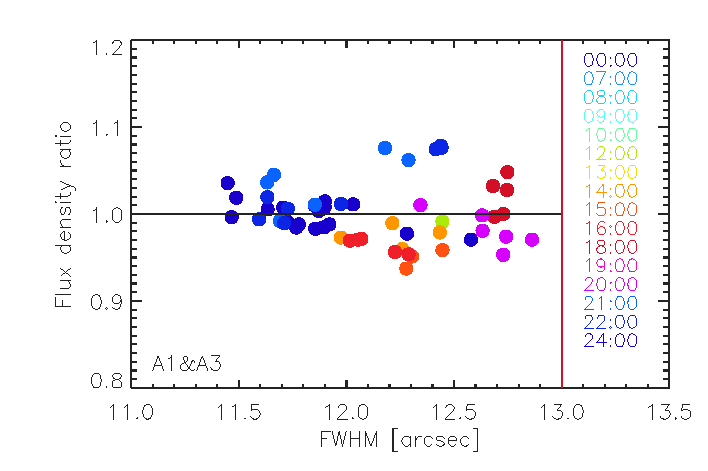
\includegraphics[clip=true,width=0.47\textwidth]{Figures/Calibration/Photocorr/plot_flux_density_ratio_primaryphotocorr_demo_1mm.pdf}
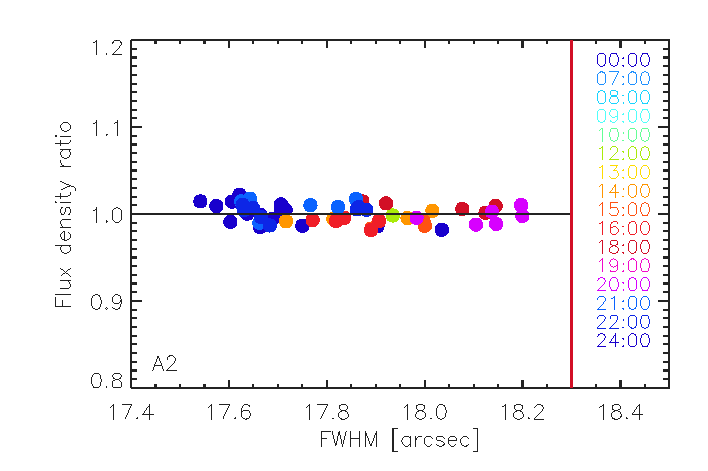
\includegraphics[clip=true,width=0.47\textwidth]{Figures/Calibration/Photocorr/plot_flux_density_ratio_primaryphotocorr_demo_a2.pdf}
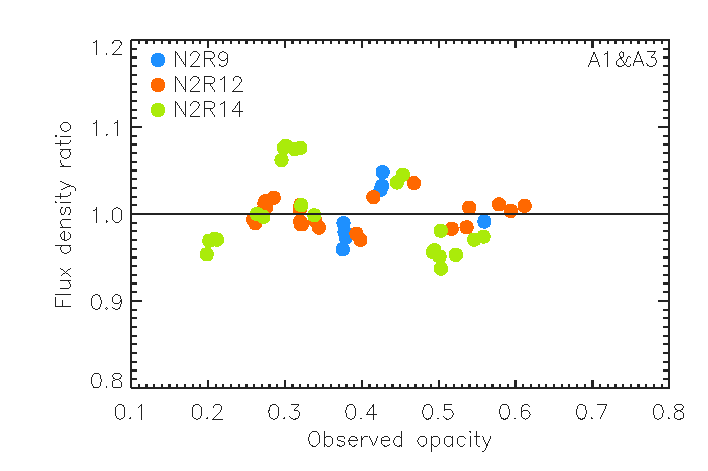
\includegraphics[clip=true,width=0.47\textwidth]{Figures/Calibration/Photocorr/plot_flux_density_ratio_obstau_primaryphotocorr_demo_1mm.pdf}
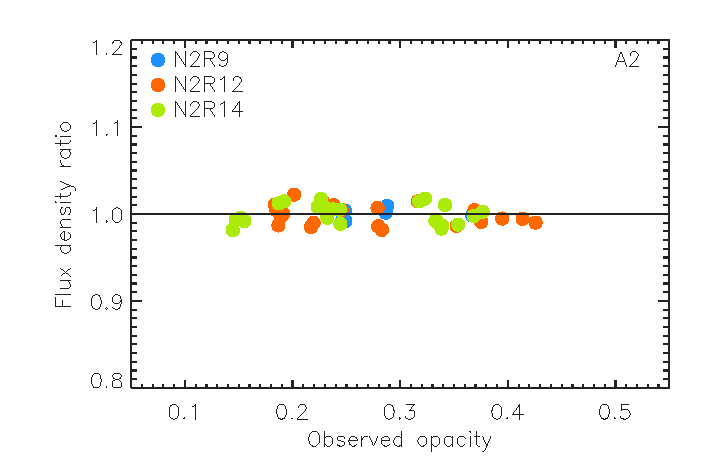
\includegraphics[clip=true,width=0.47\textwidth]{Figures/Calibration/Photocorr/plot_flux_density_ratio_obstau_primaryphotocorr_demo_a2.pdf}
\caption[Uranus flux density stability using the
  demonstration case of the beam-hardened calibration]{For the
  demonstration case of the beam-hardened calibration, 
  ratio of the Uranus measured flux densities to expectations as a
  fonction of the measured 2D Gaussian beam FWHM (top) and as a
  function of the observed opacity (bottom) for the 1mm array
  combination (left) and for array 2 (right),
  including scans acquired during N2R9, N2R12 and N2R14 campaigns. }
\label{fig:photocorr_demo_uranus_flux_fwhm}
\end{center}
\end{figure}



\subsubsection{Practical case using pointing scans}
\label{se:cal_pointings}

\addparag{ pointing-based photometric correction}

Fig.~\ref{fig:photocorr_pointing_uranus_flux_fwhm} shows the
measured-to-expected flux density ratio of Uranus observations after
calibrating using the practical case of the beam-variation
hardened calibration. 

\begin{figure}[ht!]
\begin{center}
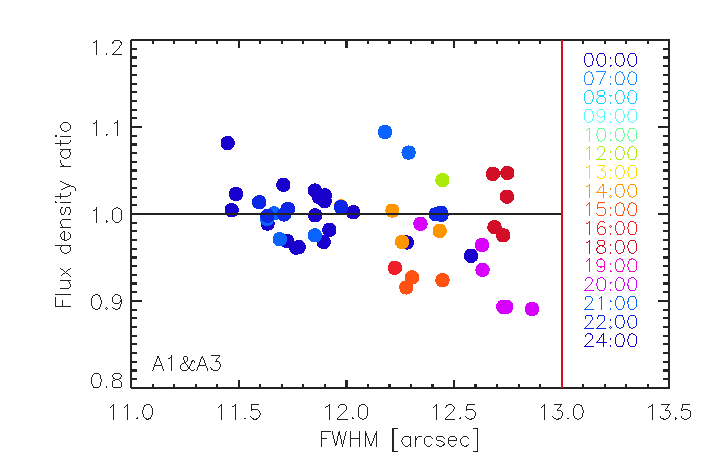
\includegraphics[clip=true,width=0.47\textwidth]{Figures/Calibration/Photocorr/plot_flux_density_ratio_primaryphotocorr_pointing_1mm.pdf}
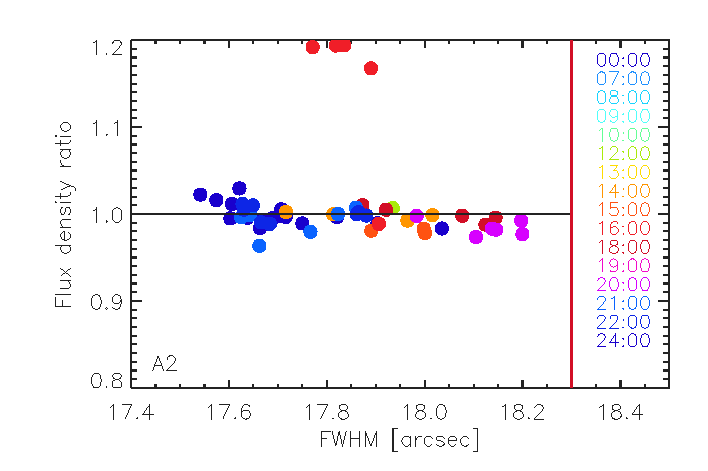
\includegraphics[clip=true,width=0.47\textwidth]{Figures/Calibration/Photocorr/plot_flux_density_ratio_primaryphotocorr_pointing_a2.pdf}
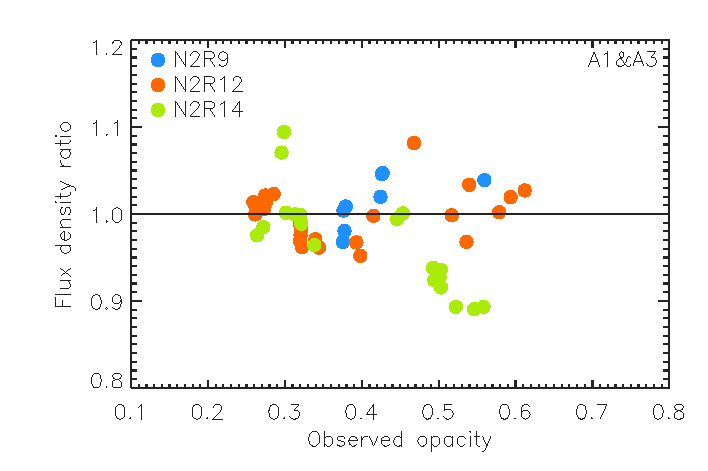
\includegraphics[clip=true,width=0.47\textwidth]{Figures/Calibration/Photocorr/plot_flux_density_ratio_obstau_primaryphotocorr_pointing_1mm.pdf}
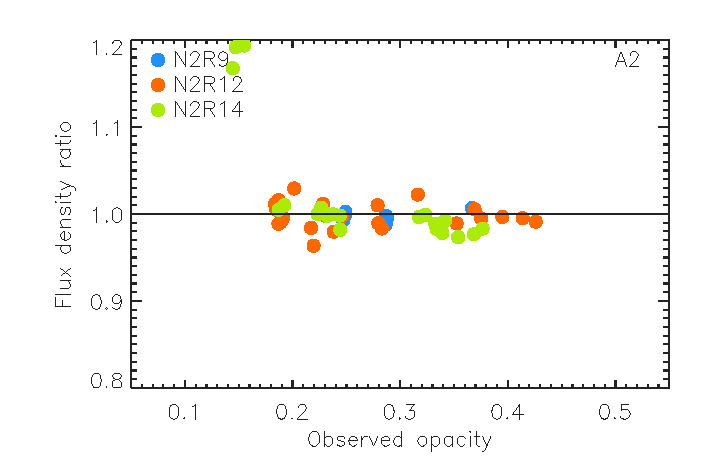
\includegraphics[clip=true,width=0.47\textwidth]{Figures/Calibration/Photocorr/plot_flux_density_ratio_obstau_primaryphotocorr_pointing_a2.pdf}
\caption[Uranus flux density stability using the
  practical case of the beam-hardened calibration]{For the
  practical case of the beam-hardened calibration, 
  ratio of the Uranus measured flux densities to expectations as a
  fonction of the measured 2D Gaussian beam FWHM (top) and as a
  function of the observed opacity (bottom) for the 1mm array
  combination (left) and for array 2 (right),
  including scans acquired during N2R9, N2R12 and N2R14 campaigns. }
\label{fig:photocorr_pointing_uranus_flux_fwhm}
\end{center}
\end{figure}

